\usepackage{amsmath,amssymb,amsthm}
\usepackage{phonetic}
\usepackage{fancyhdr}
\usepackage[pass]{geometry}
\usepackage{fontspec}
\usepackage{url}
\usepackage{booktabs}
\usepackage[table,xcdraw,dvipsnames]{xcolor}
\usepackage{algorithm}
\usepackage{algorithmicx}
\usepackage{algpseudocode}

\usepackage{wrapfig}  %% package needed for pictures to be wrapped up in text.

\usepackage{xunicode}
\usepackage{xltxtra}
%\usepackage{xgreek}
\setmainfont[Mapping=TeX-text]{Times New Roman}
\usepackage{hyperref}
\hypersetup{
    colorlinks=true,       % false: boxed links; true: colored links
    linkcolor=blue,          % color of internal links (change box color with linkbordercolor)
    citecolor=red,        % color of links to bibliography
    filecolor=magenta,      % color of file links
    urlcolor=cyan           % color of external links
}
\usepackage[Glenn]{fncychap}
\ChNameVar{\bfseries\Large}
\usepackage{tabularx}
\usepackage[normalem]{ulem}

%% myPackages (Extra)
\usepackage{enumitem}

\renewcommand{\maketitle}{
  \begin{titlepage}
    \newgeometry{left=4cm, top=2.3cm, bottom=2.3cm}

    \hbox{
      \mbox{ \hspace{-1.3cm} }
      \vrule depth 0.98 \textheight
      \mbox{ \hspace{1cm} }

        \vtop{
          \vspace{2cm}

          \begin{flushleft}
            \huge{\bf Thesis Title\\}
            \vskip3cm
            \Large  Author's name\\
            Author's Registration Number\\
            \vskip3cm

            \begin{minipage}{7.5cm}
              \begin{flushleft}
                \normalsize {\it {\bf Examination committee:}\\
                Professor's name, Department or School, Institution.\\
                Professor's name, Department or School, Institution.\\
                Professor's name, Department or School, Institution.}
              \end{flushleft}
            \end{minipage}

            \hskip0.5cm
            \begin{minipage}{6cm}
              \begin{flushleft}
                \normalsize {\it {\bf Supervisor:}\\
                Supervisor's name, Rank, \\ Department or School,\\
                Institution.\\
                }
              \end{flushleft}
            \end{minipage}

          \end{flushleft}

          \vskip6cm
          \hskip4.5cm
          \begin{minipage}{5cm}
            \begin{center}
              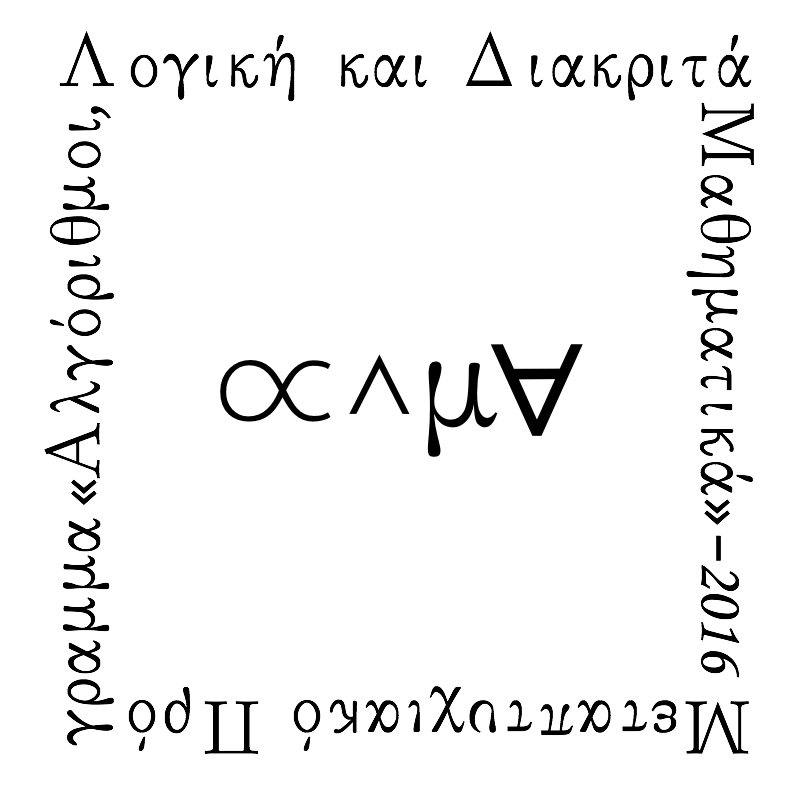
\includegraphics[width=0.8\textwidth]{alma.png}
            \end{center}
          \end{minipage}
        }
    }

 \end{titlepage}
 }

 %%%%%%%%%%%%%%%%%%%%%%%%%%%%%%%%%%%%%%%%%%%%%%%%%%%%%%%%%%%%%%%%%%%%%%%%
 %%%%%%%%%%%%%%%%%%%%%%%%%%%%%%%%%%%%%%%%%%%%%%%%%%%%%%%%%%%%%%%%%%%%%%%%

\theoremstyle{definition}
\newtheorem{ex}{}[section]
\newtheorem{definition}{Definition}[chapter]
\newtheorem{theorem}[definition]{Theorem}
\newtheorem{lemma}[definition]{Lemma}
\newtheorem{corollary}[definition]{Corollary}
\theoremstyle{remark}
\newtheorem{example}[definition]{Example}
\newtheorem{claim}[definition]{Claim}

%%%%%%%%%%%%%%%%%%%%%%%%%%%%%%%%%%%%%%%%%%%%%%%%%%%%%%%%%%%%%%%%%%%%%%%%%
%%%%%%%%%%%%%%%%%%%%%%%%%%%%%%%%%%%%%%%%%%%%%%%%%%%%%%%%%%%%%%%%%%%%%%%%%

\fancyhead[LO]{\slshape \leftmark}
\fancyhead[RE]{\slshape \rightmark}
\fancyhead[LE]{}
\fancyhead[RO]{}
\fancyfoot[LO,RE]{
\tiny{\it}}

%%%%%%%%%%%%%%%%%%%%%%%%%%%%%%%%%%%%%%%%%%%%%%%%%%%%%%%%%%%%%%%%%%%%%%%%%
%% This is for code environment, helpful.
%% (not complete, I didn't need everything)
%%%%%%%%%%%%%%%%%%%%%%%%%%%%%%%%%%%%%%%%%%%%%%%%%%%%%%%%%%%%%%%%%%%%%%%%%
\def\code#1{\texttt{#1}}
\newcommand{\easyfigure}[3]{
  \begin{figure}
    \centering
    \includegraphics[width=0.9\columnwidth,keepaspectratio]{figures/#2.#1}
    \caption{#3}
    \label{fig:#2}
  \end{figure}
}
%%%%%%%%%%%%%%%%%%%%%%%%%%%%%%%%%%%%%%%%%%%%%%%%%%%%%%%%%%%%%%%%%%%%%%%%%
%% Bitcoin font!! haha..
%%%%%%%%%%%%%%%%%%%%%%%%%%%%%%%%%%%%%%%%%%%%%%%%%%%%%%%%%%%%%%%%%%%%%%%%%
\def\bitcoin{%
  \leavevmode
  \vtop{\offinterlineskip %\bfseries
    \setbox0=\hbox{B}%
    \setbox2=\hbox to\wd0{\hfil\hskip-.03em
    \vrule height .3ex width .15ex\hskip .08em
    \vrule height .3ex width .15ex\hfil}
    \vbox{\copy2\box0}\box2}}
